\section{Final Application}
The final application is costist of five different pages that are described in the following sections.

\subsection{Managing Subprocesses}
The \srgui possesses a crucial capability of initiating, terminating, and monitoring external Python (\py) applications that run on the \jx system.
Currently, the \srgui manages two distinct \py applications.
One handles the \gls{ptp} Deamons responsible for synchronizing the \cams, while the other handles the \gls{sensorpipeline}.
Each application has its own dedicated page within the \srgui interface, as depicted in Figure \ref{fig:gui_map}.
Separating these subprocesses is beneficial because whenever a \gls{ptp} Deamon is stopped and restarted, the \cams lose synchronization, requiring an extended period to resynchronize.
The started processes are encapsulated within a custom wrapper class and managed by a process manager.
This manager ensures that only one instance of each process runs at a time, facilitates graceful shutdowns, and directs the output from \code{stderr} and \code{stdout} to the respective process log topics, making them readabe in the \srgui as shown.

\begin{figure}[H]
    \centering
    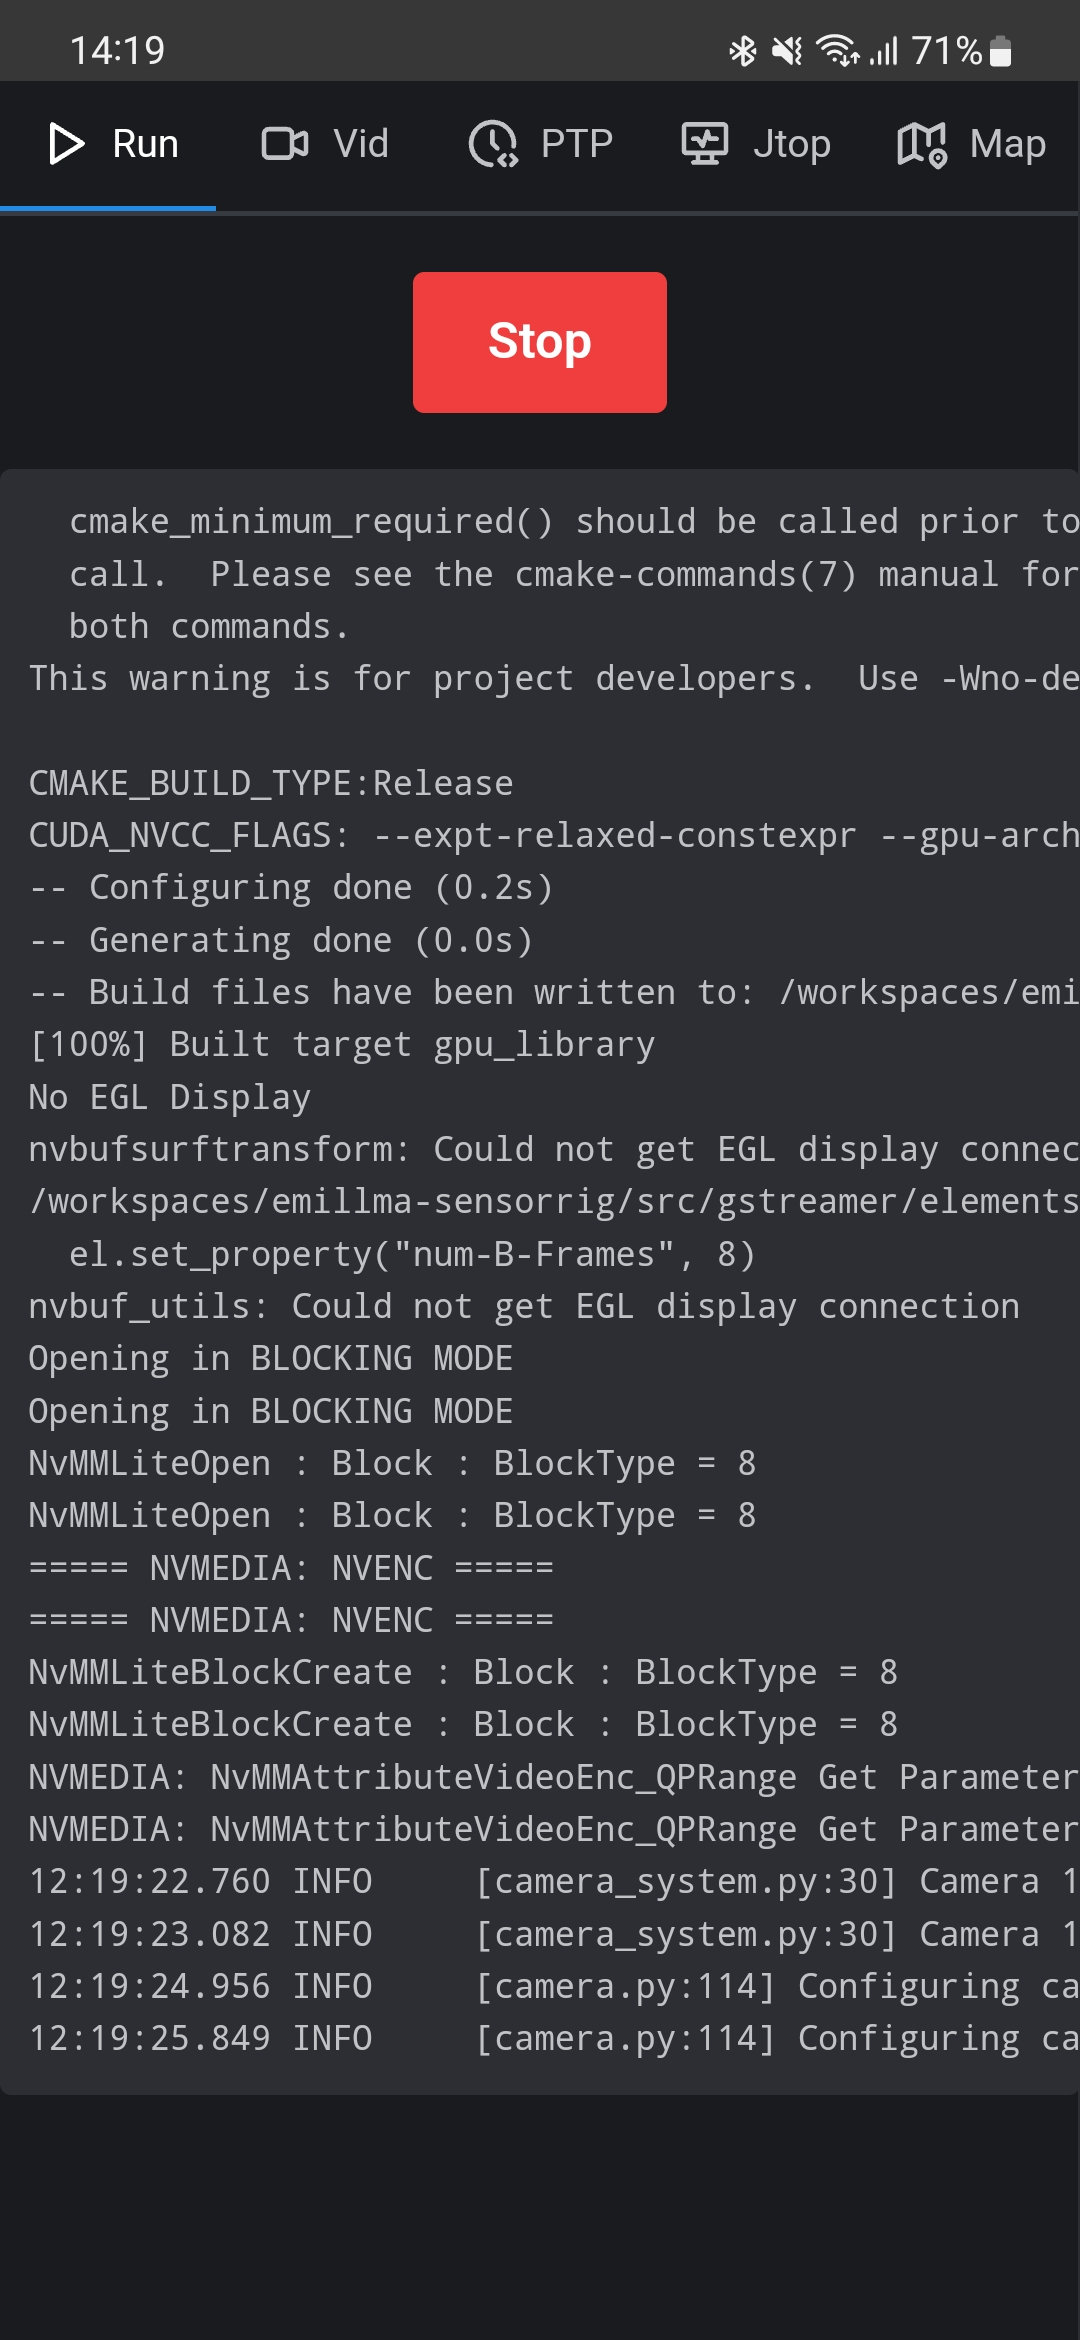
\includegraphics[width=.48\textwidth]{figures/gui/run.jpg}
    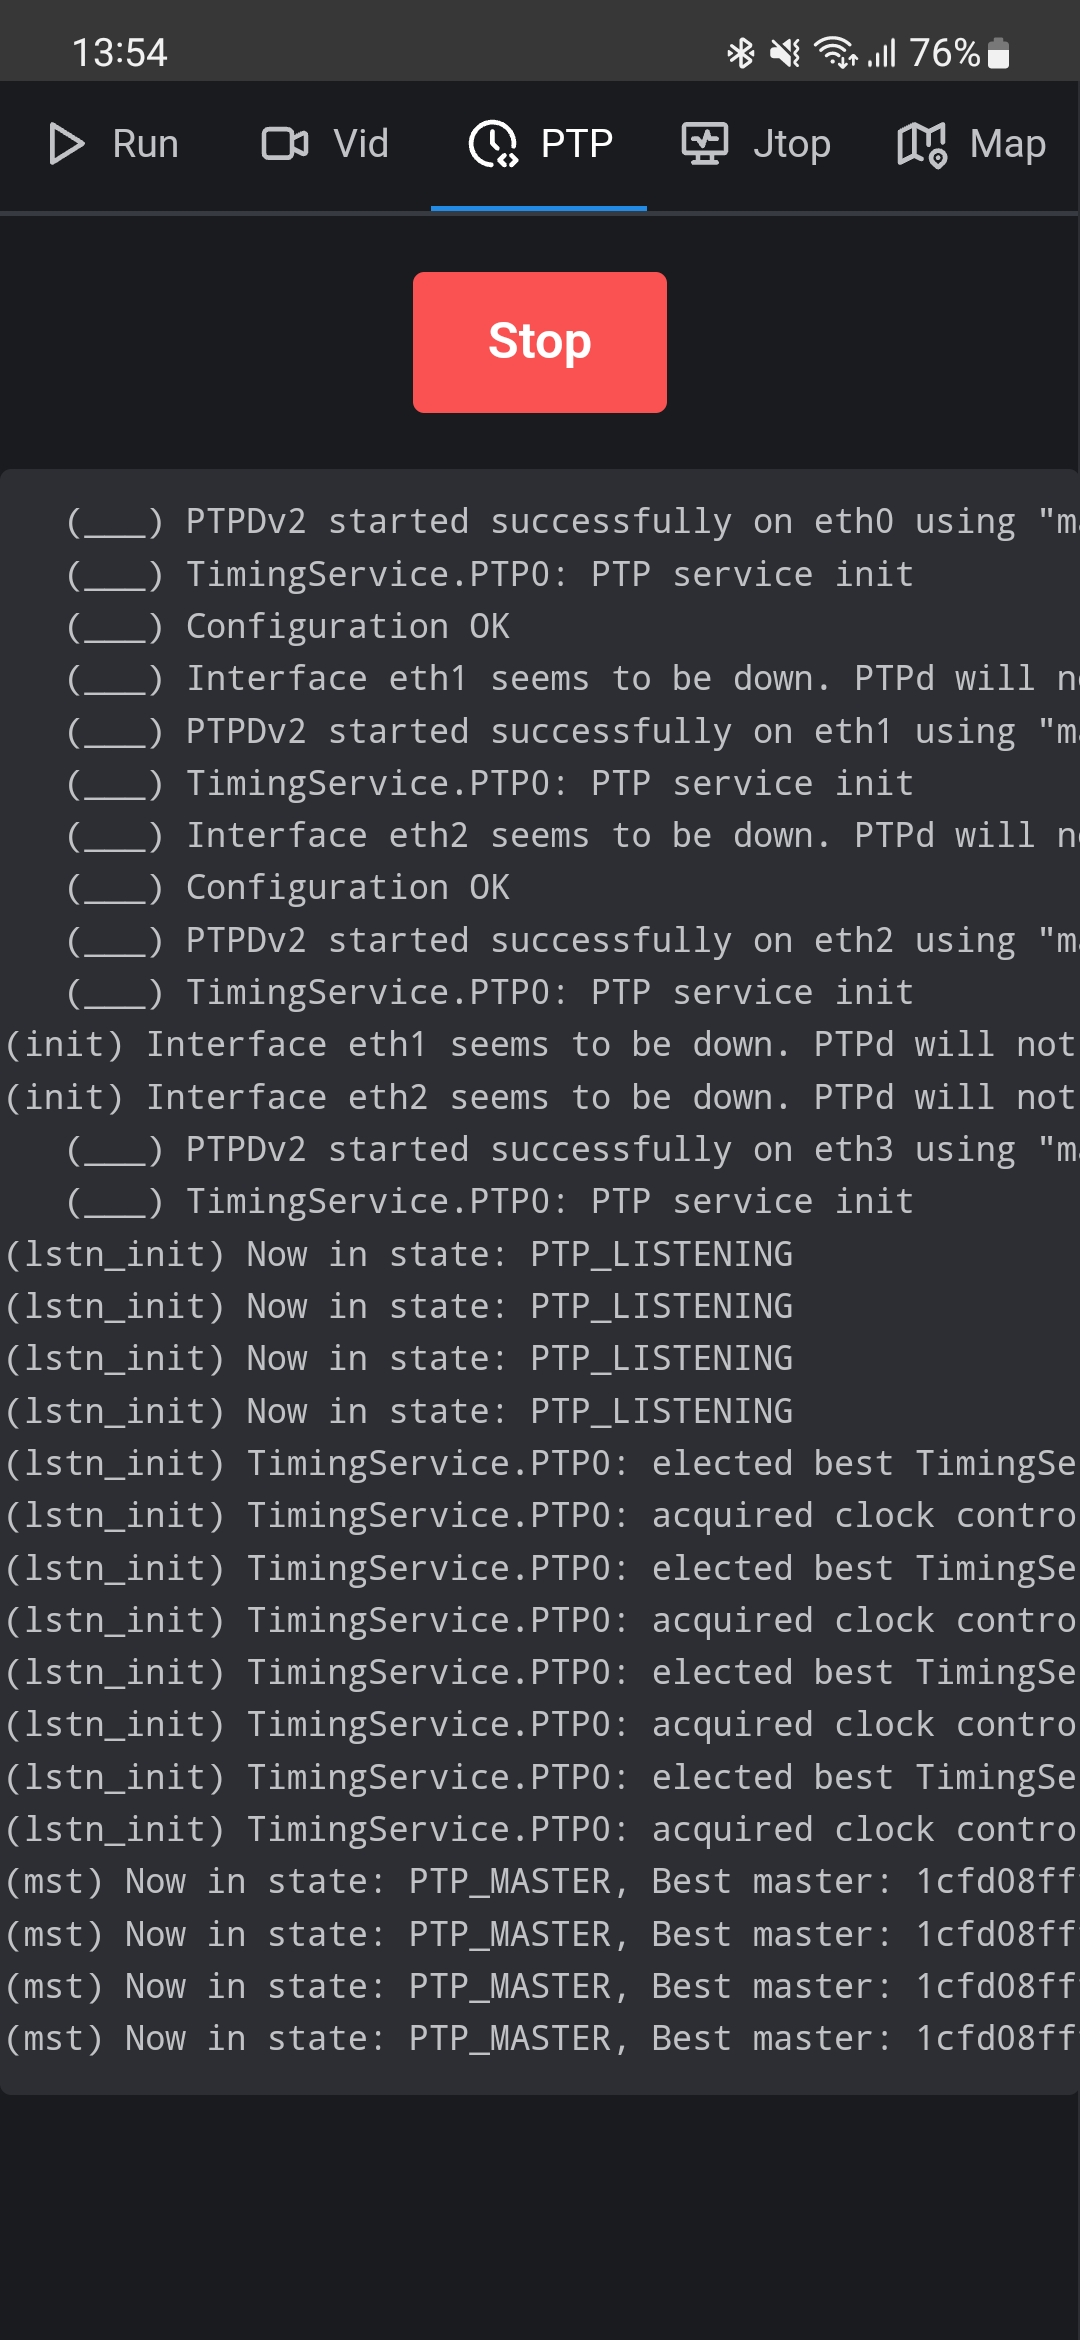
\includegraphics[width=.48\textwidth]{figures/gui/ptp.jpg}
    \caption{The \textit{Run} and \textit{PTP} page of \srgui used to start, stop and monitor the two \py applications.}
    \label{fig:gui_map}
\end{figure}

